%============================================================
%  PrepPilot — AI Interview Prep Bot : Project Report
%  Compile with pdfLaTeX (Overleaf-ready). Run twice so the
%  table of contents resolves.
%  >>> Fill the placeholders marked with [...] on the title page.
%============================================================
\documentclass[11pt,a4paper]{article}

\usepackage[utf8]{inputenc}
\usepackage[T1]{fontenc}
\usepackage[a4paper,margin=1in]{geometry}
\usepackage{graphicx}
\usepackage{xcolor}
\usepackage{booktabs}
\usepackage{tabularx}
\usepackage{enumitem}
\usepackage{listings}
\usepackage{tikz}
\usetikzlibrary{positioning, arrows.meta}
\usepackage[hidelinks]{hyperref}
\hypersetup{colorlinks=true, linkcolor=black, urlcolor=blue!60!black, citecolor=black}

%------------------ colours & code style ------------------
\definecolor{codebg}{RGB}{245,246,250}
\definecolor{codekw}{RGB}{99,102,241}
\definecolor{codestr}{RGB}{22,140,90}
\definecolor{codecmt}{RGB}{130,135,150}
\definecolor{accent}{RGB}{99,102,241}

\lstset{
  backgroundcolor=\color{codebg},
  basicstyle=\ttfamily\footnotesize,
  keywordstyle=\color{codekw}\bfseries,
  stringstyle=\color{codestr},
  commentstyle=\color{codecmt}\itshape,
  breaklines=true,
  frame=single,
  rulecolor=\color{gray!30},
  numbers=left,
  numberstyle=\tiny\color{gray},
  numbersep=8pt,
  showstringspaces=false,
  tabsize=2,
  captionpos=b,
  xleftmargin=16pt,
}

\newcommand{\code}[1]{\texttt{#1}}

\begin{document}

%====================== TITLE PAGE ======================
\begin{titlepage}
\centering
\vspace*{0.5cm}

{\large \textbf{[Your College / University Name]}\par}
\vspace{0.2cm}
{\normalsize Department of [Your Department]\par}

\vspace{2.2cm}
{\Huge \textbf{PrepPilot}\par}
\vspace{0.4cm}
{\LARGE An AI-Powered Mock Interview System\par}
\vspace{0.3cm}
{\large (AI Interview Prep Bot)\par}

\vspace{1.6cm}
{\large A Project Report submitted in partial fulfillment\\
of the requirements for the course\\
\textbf{[Course Name / Code]}\par}

\vspace{2.0cm}
\begin{tabular}{rl}
\textbf{Submitted by:} & [Your Name] \\[4pt]
\textbf{Roll No.:} & [Your Roll Number] \\[4pt]
\textbf{Guide:} & [Professor / Guide Name] \\[4pt]
\end{tabular}

\vfill
{\large \textbf{Academic Year 2025--2026}\par}
\vspace{0.4cm}
% \includegraphics[width=0.18\textwidth]{college_logo.png}  % optional: add your logo
\end{titlepage}

%====================== ABSTRACT ======================
\section*{Abstract}
\addcontentsline{toc}{section}{Abstract}
\textbf{PrepPilot} is an AI-powered web application that lets a candidate practise
job interviews on demand. The user selects a target role, experience level and
interview type; an AI interviewer then asks relevant questions one at a time. The
candidate answers either by \emph{typing} or by \emph{speaking} (the voice is
transcribed automatically), and receives an \emph{instant, scored evaluation} of
every answer, including strengths, areas to improve and a model answer. At the end
of the session a consolidated performance report is produced with an overall score,
a summary and targeted preparation tips.

The system is built as a decoupled client--server application: a \textbf{FastAPI}
backend exposes a small REST API, and a \textbf{React} single-page application
provides the user interface. The intelligence is powered by a Large Language Model
(LLM) served through \textbf{Groq} for question generation, answer evaluation and
report synthesis, while \textbf{Groq Whisper} performs speech-to-text for voice
answers. The LLM layer is provider-agnostic and can be switched to Google Gemini,
OpenAI or a local Ollama model through configuration alone.

\newpage
\tableofcontents
\newpage

%====================== INTRODUCTION ======================
\section{Introduction}

\subsection{Overview}
Interviews are a decisive step in every hiring process, yet most candidates get
very few opportunities to practise under realistic conditions and receive honest,
structured feedback. Human mock interviews are effective but expensive, hard to
schedule and inconsistent. PrepPilot addresses this gap by acting as an always-available
AI interviewer that conducts a tailored mock interview and provides objective,
immediate feedback.

\subsection{Problem Statement}
To design and build a web application that can (a) generate role-specific interview
questions, (b) accept candidate answers through both text and voice, (c) evaluate each
answer and score it, and (d) summarise the candidate's overall performance, without
requiring any human interviewer.

\subsection{Objectives}
\begin{itemize}[leftmargin=1.4em]
  \item Generate interview questions tailored to a chosen role, difficulty level and
        interview type (technical, behavioural or mixed), optionally guided by a job
        description.
  \item Support \textbf{voice answers} using automatic speech recognition, in addition
        to typed answers.
  \item Provide \textbf{instant per-answer feedback}: a score out of 10, strengths,
        improvements and a model answer.
  \item Produce a \textbf{final report} with an overall score, summary, strengths,
        weaknesses and preparation tips.
  \item Keep the system \textbf{fast and free} to run by using an efficient hosted LLM.
\end{itemize}

\subsection{Scope}
The current version is a single-user, session-based web application. Interview
sessions are held in server memory for the duration of a session. The project focuses
on the core interview-practice loop and feedback generation; it does not include user
accounts or long-term history storage, which are identified as future work.

%====================== TECHNOLOGIES ======================
\section{Technologies Used}

\begin{table}[h]
\centering
\renewcommand{\arraystretch}{1.25}
\begin{tabularx}{\textwidth}{@{}l l X@{}}
\toprule
\textbf{Layer} & \textbf{Technology} & \textbf{Purpose} \\
\midrule
Backend framework & FastAPI + Uvicorn & Asynchronous REST API server (Python) \\
Data validation   & Pydantic          & Request/response schema validation \\
LLM access        & OpenAI Python SDK & Unified client for OpenAI-compatible APIs \\
LLM provider      & Groq (\code{openai/gpt-oss-120b}) & Question generation, evaluation, reporting \\
Speech-to-text    & Groq Whisper (\code{whisper-large-v3-turbo}) & Transcribing voice answers \\
Text-to-speech    & Web Speech API    & Reading questions aloud (in the browser) \\
Voice capture     & MediaRecorder API & Recording the candidate's spoken answer \\
Frontend          & React 18 + Vite   & Single-page user interface \\
Icons             & lucide-react      & UI iconography \\
Config            & python-dotenv     & Environment-based configuration \\
\bottomrule
\end{tabularx}
\caption{Technology stack}
\end{table}

A notable design decision is that PrepPilot requires \emph{no} vector database or
embedding model: unlike a Retrieval-Augmented Generation (RAG) system, it is a purely
\emph{generative} question-and-evaluation application. This keeps the dependency
footprint small and the installation lightweight (no PyTorch).

%====================== ARCHITECTURE ======================
\section{System Architecture}

PrepPilot follows a standard three-tier architecture. The browser-based React client
communicates with the FastAPI backend over a JSON REST API; the backend in turn calls
the Groq cloud for all AI operations. Session state lives in the backend's memory.

\begin{figure}[h]
\centering
\resizebox{\textwidth}{!}{%
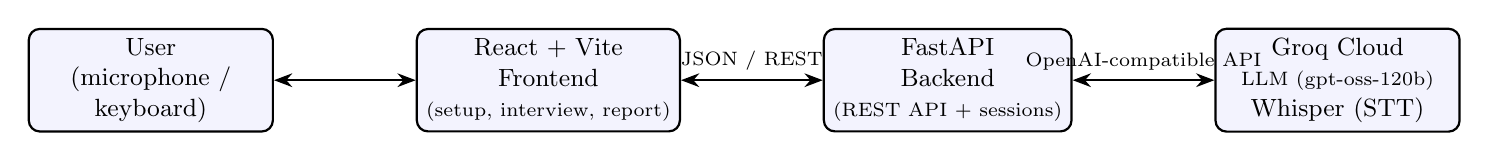
\begin{tikzpicture}[node distance=1.8cm, every node/.style={font=\small}]
  \tikzset{box/.style={draw, rounded corners, align=center, minimum height=1.3cm, minimum width=3.1cm, fill=accent!8, thick}}
  \node[box] (user) {User\\ (microphone /\\ keyboard)};
  \node[box, right=of user] (fe) {React + Vite\\ Frontend\\ \scriptsize (setup, interview, report)};
  \node[box, right=of fe] (be) {FastAPI\\ Backend\\ \scriptsize (REST API + sessions)};
  \node[box, right=of be] (groq) {Groq Cloud\\ \scriptsize LLM (gpt-oss-120b)\\ Whisper (STT)};
  \draw[{Stealth}-{Stealth}, thick] (user) -- (fe);
  \draw[{Stealth}-{Stealth}, thick] (fe) -- node[above]{\scriptsize JSON / REST} (be);
  \draw[{Stealth}-{Stealth}, thick] (be) -- node[above]{\scriptsize OpenAI-compatible API} (groq);
\end{tikzpicture}%
}
\caption{High-level architecture of PrepPilot}
\end{figure}

\subsection{Data Flow}
\begin{enumerate}[leftmargin=1.6em]
  \item The user configures the interview (role, level, type, number of questions,
        optional job description) and starts the session.
  \item The frontend calls \code{POST /api/start}; the backend asks the LLM to generate
        the first question and returns it with a session identifier.
  \item The user answers. For a voice answer, the browser records audio and uploads it
        to \code{POST /api/transcribe}, which returns the transcribed text (editable
        before submission).
  \item The answer is sent to \code{POST /api/answer}. The backend asks the LLM to
        evaluate it, stores the result, and generates the next question.
  \item Steps 3--4 repeat until all questions are answered.
  \item The frontend requests \code{GET /api/report/\{id\}}; the backend asks the LLM to
        synthesise a final report from the full transcript.
\end{enumerate}

%====================== IMPLEMENTATION ======================
\section{Implementation}

\subsection{Backend Modules}
The backend is organised into focused modules under the \code{backend/} package:

\begin{table}[h]
\centering
\renewcommand{\arraystretch}{1.2}
\begin{tabularx}{\textwidth}{@{}l X@{}}
\toprule
\textbf{Module} & \textbf{Responsibility} \\
\midrule
\code{config.py}     & Loads settings from the \code{.env} file (provider, model, keys). \\
\code{schemas.py}    & Pydantic request/response models for all endpoints. \\
\code{store.py}      & In-memory interview-session store. \\
\code{llm\_client.py} & Provider-agnostic LLM client; question generation, answer
                        evaluation and report generation. \\
\code{stt.py}        & Speech-to-text for voice answers via Groq Whisper. \\
\code{routes.py}     & FastAPI route handlers (the REST endpoints). \\
\code{main.py}       & Application entry point, CORS and error handling. \\
\bottomrule
\end{tabularx}
\caption{Backend module responsibilities}
\end{table}

\subsection{Provider-Agnostic LLM Client}
All AI providers used (Groq, Gemini, OpenAI, Ollama) expose an OpenAI-compatible
Chat Completions API. The client therefore uses a single SDK and simply changes the
base URL and API key based on configuration, so the provider can be swapped from the
\code{.env} file without any code change.

\begin{lstlisting}[language=Python, caption={Resolving the provider endpoint (simplified)}]
_PROVIDER_BASE_URLS = {
    "groq":   "https://api.groq.com/openai/v1",
    "gemini": "https://generativelanguage.googleapis.com/v1beta/openai/",
    "openai": None,
    "ollama": "http://localhost:11434/v1",
}

def get_client():
    base_url = settings.LLM_BASE_URL or _PROVIDER_BASE_URLS[settings.LLM_PROVIDER]
    return OpenAI(api_key=resolve_api_key(), base_url=base_url, timeout=90.0)
\end{lstlisting}

To tolerate the occasional rate-limit or "high demand" response from a free-tier
provider, every LLM call is wrapped in a small retry with back-off on transient errors.

\subsection{Answer Evaluation}
The core of the application is the evaluation step. The LLM is instructed to act as a
seasoned interviewer and to return strictly-formatted JSON, which the backend parses
and validates. This yields a numeric score together with structured feedback.

\begin{lstlisting}[language=Python, caption={Answer-evaluation prompt (abridged)}]
messages = [
  {"role": "system", "content":
     "You are a seasoned interviewer evaluating a candidate's answer for a "
     f"{role} role. Be fair, specific and constructive. Respond with STRICT "
     'JSON: {"score": <0-10>, "verdict": "...", "strengths": [...], '
     '"improvements": [...], "ideal_answer": "..."}.'},
  {"role": "user", "content": f"Question:\n{question}\n\nAnswer:\n{answer}"},
]
raw = chat(messages, json_mode=True)
evaluation = safe_json(raw)   # parsed + range-checked
\end{lstlisting}

\subsection{Voice Answers}
On the frontend, the browser's \code{MediaRecorder} API captures the candidate's spoken
answer as an audio blob, which is uploaded to the backend and transcribed with Groq
Whisper. The transcribed text is placed in the answer box, where the candidate can
review and edit it before submitting.

\begin{lstlisting}[language=JavaScript, caption={Recording and transcribing a voice answer (abridged)}]
const stream = await navigator.mediaDevices.getUserMedia({ audio: true })
const mr = new MediaRecorder(stream)
mr.ondataavailable = (e) => chunks.push(e.data)
mr.onstop = async () => {
  const blob = new Blob(chunks, { type: 'audio/webm' })
  const form = new FormData(); form.append('file', blob, 'answer.webm')
  const { text } = await (await fetch(API + '/api/transcribe',
                      { method: 'POST', body: form })).json()
  setAnswer((a) => (a ? a + ' ' : '') + text)
}
mr.start()
\end{lstlisting}

Questions can also be read aloud using the browser's Web Speech API
(\code{speechSynthesis}), giving the practice session a more realistic feel.

\subsection{Frontend}
The React application is a single page with three stages: \textbf{Setup}
(choose role, level, type, number of questions, optional job description),
\textbf{Interview} (question, answer box, microphone, per-answer feedback) and
\textbf{Report} (overall score and analysis). The application communicates with the
backend purely through \code{fetch} calls to the REST API.

%====================== API ======================
\section{API Reference}

\begin{table}[h]
\centering
\renewcommand{\arraystretch}{1.25}
\begin{tabularx}{\textwidth}{@{}l l X@{}}
\toprule
\textbf{Method} & \textbf{Endpoint} & \textbf{Description} \\
\midrule
GET  & \code{/api/health}            & Service status and configured model. \\
POST & \code{/api/start}             & Start a session; returns the first question. \\
POST & \code{/api/answer}            & Evaluate an answer; returns feedback and the next question. \\
POST & \code{/api/transcribe}        & Transcribe an uploaded voice answer to text. \\
GET  & \code{/api/report/\{id\}}      & Generate the final performance report. \\
\bottomrule
\end{tabularx}
\caption{REST API endpoints}
\end{table}

%====================== FEATURES ======================
\section{Features}
\begin{itemize}[leftmargin=1.4em]
  \item \textbf{Role-based questions} tailored to role, level (Junior/Mid/Senior) and
        type (Technical/Behavioural/Mixed).
  \item \textbf{Job-description aware}: pasting a JD yields more targeted questions.
  \item \textbf{Voice or text answers}, with automatic, editable transcription.
  \item \textbf{Spoken questions} via text-to-speech (optional).
  \item \textbf{Instant scored feedback} per answer: score out of 10, strengths,
        improvements and a model answer.
  \item \textbf{Final report}: overall score, summary, strengths, weaknesses,
        preparation tips and a question-by-question review.
  \item \textbf{Provider-agnostic AI}: switch between Groq, Gemini, OpenAI or a local
        Ollama model from configuration.
\end{itemize}

%====================== TESTING ======================
\section{Testing and Results}
The complete interview loop was tested end-to-end through both the REST API and the
user interface. Key observations:
\begin{itemize}[leftmargin=1.4em]
  \item Question generation produced relevant, role-appropriate questions
        (e.g., for a Frontend Developer: \emph{``How would you implement a debounced
        search input in React and why is debouncing important?''}).
  \item The evaluator behaved discriminatively: a strong, on-topic answer received
        \textbf{9/10} with specific strengths and improvements, while an answer that did
        not match the question was correctly scored \textbf{1/10} with an explanation of
        the mismatch --- confirming that the model genuinely assesses the content.
  \item The final report aggregated per-question scores into an overall score with a
        written summary and actionable tips.
  \item Voice answers were transcribed and inserted into the answer box for review.
\end{itemize}

\subsection*{Screenshots}
Add your own screenshots here (run the app, capture the screens, and place the image
files next to this report). Example usage:
\begin{lstlisting}[numbers=none]
\begin{figure}[h]
  \centering
  \includegraphics[width=0.8\textwidth]{setup_screen.png}
  \caption{Interview setup screen}
\end{figure}
\end{lstlisting}

%====================== LIMITATIONS ======================
\section{Limitations}
\begin{itemize}[leftmargin=1.4em]
  \item Interview sessions are stored in memory and are lost when the backend restarts.
  \item The application requires an internet connection and a valid (free) API key for
        the chosen LLM provider.
  \item Voice recording requires microphone permission and a secure context
        (it works on \code{localhost}).
  \item Free API tiers are subject to rate limits; very high usage may be throttled.
\end{itemize}

%====================== FUTURE SCOPE ======================
\section{Future Scope}
\begin{itemize}[leftmargin=1.4em]
  \item User accounts with persistent interview history and progress tracking.
  \item Resume upload and parsing to automatically tailor questions.
  \item An analytics dashboard showing improvement over time.
  \item Adaptive difficulty that reacts to the quality of previous answers.
  \item Video interview mode with body-language / confidence cues.
  \item One-click export of the final report to PDF.
\end{itemize}

%====================== CONCLUSION ======================
\section{Conclusion}
PrepPilot demonstrates how a modern Large Language Model can be applied to a practical,
high-value problem: interview preparation. By combining role-aware question generation,
voice-enabled answering and structured, scored feedback, the system offers a realistic
and genuinely useful practice experience. Its clean, provider-agnostic architecture
keeps it lightweight, inexpensive to run and easy to extend, making it a strong
foundation for the future enhancements outlined above.

%====================== REFERENCES ======================
\begin{thebibliography}{9}
\bibitem{fastapi} FastAPI Documentation. \url{https://fastapi.tiangolo.com/}
\bibitem{react} React Documentation. \url{https://react.dev/}
\bibitem{vite} Vite Documentation. \url{https://vitejs.dev/}
\bibitem{groq} Groq API Documentation. \url{https://console.groq.com/docs}
\bibitem{whisper} Radford, A. et al. \textit{Robust Speech Recognition via Large-Scale
  Weak Supervision} (Whisper), OpenAI, 2022.
\bibitem{openai} OpenAI Python SDK. \url{https://github.com/openai/openai-python}
\end{thebibliography}

\end{document}
